\documentclass[letterpaper, 10 pt, conference]{ieeeconf}  % Comment this line out if you need a4paper

%\documentclass[a4paper, 10pt, conference]{ieeeconf}      % Use this line for a4 paper

\IEEEoverridecommandlockouts                              % This command is only needed if 
                                                          % you want to use the \thanks command

\overrideIEEEmargins                                      % Needed to meet printer requirements.

%In case you encounter the following error:
%Error 1010 The PDF file may be corrupt (unable to open PDF file) OR
%Error 1000 An error occurred while parsing a contents stream. Unable to analyze the PDF file.
%This is a known problem with pdfLaTeX conversion filter. The file cannot be opened with acrobat reader
%Please use one of the alternatives below to circumvent this error by uncommenting one or the other
%\pdfobjcompresslevel=0
%\pdfminorversion=4

% See the \addtolength command later in the file to balance the column lengths
% on the last page of the document

% The following packages can be found on http:\\www.ctan.org
%\usepackage{graphics} % for pdf, bitmapped graphics files
%\usepackage{epsfig} % for postscript graphics files
%\usepackage{mathptmx} % assumes new font selection scheme installed
%\usepackage{times} % assumes new font selection scheme installed
%\usepackage{amsmath} % assumes amsmath package installed
\usepackage{amssymb}  % assumes amsmath package installed
\usepackage{amscd,amsmath}
\usepackage{amsfonts}
\usepackage{biblatex}
\usepackage{csvsimple}
\usepackage{pgfplots}
\usepackage{pgfplotstable}
\usepackage{hyperref}
\usepackage{algorithm}
\usepackage{algpseudocode}
\usepackage{rotating}
\usepackage{gensymb}
%\pgfplotsset{compat=1.7}
\usepackage{graphicx}
\usepackage{import}
\usepackage{placeins}
\usepackage{multirow}
\usepackage{booktabs}
\usepackage{xcolor}
\usepackage{pgf}
\usepackage{subcaption}
%\usepackage[maxfloats=256]{morefloats}
%\maxdeadcycles=1000
%\usepgfplotslibrary{external} 
%\tikzexternalize

\newcommand\norm[1]{\left\lVert#1\right\rVert}

\title{\LARGE \bf
Fault Detection of Sun Reflection to Increase Estimation Accuracy of Satellite Attitude
}


\author{Louw UJ$^{1}$, Jordaan HW$^{2}$, Schoeman JC$^{3}$% <-this % stops a space
\thanks{*This work was not supported by any organization}% <-this % stops a space
\thanks{$^{1}$Louw UJ is with Faculty of Electronic \& Electrical Engineering, Electronic System            Laboratory, University of Stellenbosch, Stellenbosch Central, Stellenbosch, 7600
        {\tt\small louwuj@gmail.com}}%
}

\addbibresource{bibliography.bib} 

\begin{document}



\maketitle
\thispagestyle{empty}
\pagestyle{empty}


%%%%%%%%%%%%%%%%%%%%%%%%%%%%%%%%%%%%%%%%%%%%%%%%%%%%%%%%%%%%%%%%%%%%%%%%%%%%%%%%
\begin{abstract}

The Kalman Filter is a state estimator that is often used in attitude determination of satellites. A Kalman filter is highly sensitive to anomalies that occur in sensors. A good example of this is the reflection of a solar panel on a sun sensor that changes the perceived sun vector. This in term influences the estimation of the attitude by the kalman filter and consequently the control of the satellite. Detecting anomalies in sensors and omitting the sensor reading from the measurement update of the Kalman Filter increases the stability and reliability of the Kalman filter for satellite attitude determination. However detecting when an anomaly occurs is difficult and an accuracy of more than $99\%$ is required to produce satisfactory results.

\emph{keywords} --- anomaly detection, Kalman filter, machine learning, sun reflection, satellites

\end{abstract}


%%%%%%%%%%%%%%%%%%%%%%%%%%%%%%%%%%%%%%%%%%%%%%%%%%%%%%%%%%%%%%%%%%%%%%%%%%%%%%%%
\section{INTRODUCTION}
For many satellite missions the attitude determination is of high importance. A mission that requires earth following during eclipse and otherwise sun following for solar charging requires accurate attitude estimation. The current state vector of the system can not be determined with only the use of models or sensors. Since the sensors contains noise and the mathematical model does not include certain disturbances of the actual system. Therefore a probabilistic approach can be used to determine the attitude from both the model and the sensors. This probabilistic approach is done with the use of an extended kalman filter (\emph{EKF}). 

The focus of this article is the attitude determination and control system, \emph{ADCS}, of the satellite. This system is demonstrated in Figure~\ref{fig:System_Diagram}, where the basic ADCS excludes the fault detection, isolation and recovery, \emph{FDIR}, and feature extraction. The FDIR for sensors receive the sensor measurements and the feature extractions as inputs and outputs the recovery method if it is required. 

The EKF is a method which incorporates a physics based model of the satellite dynamics as well as using sensor fusion and measurement updates to ensure accurate estimation. The sensor measurements that are used for the measurement update, are the sensors that provide a modelled vector in the orbit-referenced coordinate, \emph{ORC}, frame as well as a measured vector in the satellite body coordinate, \emph{SBC}, frame. The sensors used for the measurement update according to the general satellite design is a magnetometer, sun sensor and nadir sensor. The noise of the measurements and the noise of the system is incorporated in the EKF model to ensure stability and reliable estimation. The general principal for measurement updates, is to update the EKF from the least to the most reliable sensor measurements. The error between the modelled and measured vectors are used to update the EKF. The EKF and the specific configuration thereof for satellites can be researched further~\cite{JansevanVuuren2015}. 

The problem with an EKF is when the sensors do not follow their modelled vector. Slight deviations thereof won't have significant effects, but anomalies such as failed sensors can cause the EKF to become unstable. Consequently, we want to be able to recover from failed sensors. The frequency of the anomaly occurrence can also influence the stability of the Kalman filter. Therefore we opted to use sun reflection from the solar panel on sun sensors as our modelled anomaly. This is because of the accurate modelling for sun reflection. This is a real problem in the satellite industry that can be isolated with changes in the satellite design to ensure that sun reflection does not occur on the sun sensor.

This anomaly also requires autonomous decision making to ensure sun facing control. This cannot be done by the ground station during orbit, unless the control system is dramatically changed after the anomaly is detected by the ground station. Therefore we aim to design a fault detection, isolation and recovery system for the specific use case of a mission that requires earth following during eclipse and sun following otherwise on a generic small satellite design as seen in Figure~\ref{fig:CubeSat}.

\begin{figure*}[h!b!t]
	\centering
	\def\svgwidth{14cm}
	\import{Figures/}{Control_Diagram.pdf_tex}
	\caption{System Diagram}
	\label{fig:System_Diagram}
\end{figure*}

\subsection{Related Work}
Sun reflection is not a new problem and has consequently been researched thoroughly. Hardware solutions to sun reflection have been developed with the use of digital sun sensors that can discriminate between direct sunlight and reflected sunlight. These digital sun sensors however, are not as accurate as many other analog sun sensors. There is also a long list of research that has been done with regards to sensor fault detection (as seen in \cite{wang2019adaptive}). One of the most relevant articles is done by \textcite{wang2019adaptive}, and proposed a adaptive unscented Kalman filter for sensor fault estimation and isolation. The results thereof seems promising and are based on dramatical changes in the measurements. However, the research is not based on failures such as sun reflection, the results are based on drastic modelled failures. Therefore, future work will be to use the algorithm developed by \textcite{wang2019adaptive} to test the response thereof on sun reflection, noting that sun reflection occurs regularly during the sunlight phase of the orbit.

Other research that is used for feature extraction in this article is based on research done by \textcite{DeSilva2020}. Fault prediction is done by implementing an innovative moving average, determined by the error estimated with dynamic mode decomposition, \emph{DMD}, and a kalman filter, as an input to a predictive model --- decision tree. The method however is adjusted for our use case to be a linear regression model instead of DMD.

\subsection{Preliminaries}
The details of satellite dynamics will not be discussed in this article, however it must be noted that the orbit-reference coordinate and satellite body coordinate frame will be referred to as \emph{ORC} and \emph{SBC} respectively. General notation of this article is matrices in upper case and bold, vectors in lower case and bold and scalars as lower or upper case but not in bold as illustrated below.
\begin{itemize}
	\item{\makebox[1.5cm]{Matrix\hfill} $\mathbf{A}$}
	\item{\makebox[1.5cm]{Vector\hfill} $\mathbf{a} = \begin{bmatrix} 
			x & y & z
		\end{bmatrix}$}
	\item{\makebox[1.5cm]{Scalar\hfill} $a$ or $A$}
\end{itemize}

This will be the notation throughout this article unless specified otherwise. 

\section{Reflection}
\label{section:Reflection}
The reflection anomaly is modelled for the specific shape and design of the cubesat as shown in Figure~\ref{fig:CubeSat}.

\begin{figure}[!htb]
	\centering
	\def\svgwidth{7cm}
	\import{Figures/}{ReflectionModel.pdf_tex}
	\caption{Cube Sat}
	\label{fig:CubeSat}
\end{figure}

\begin{figure*}[!hbt]
	\centering
	\def\svgwidth{7cm}
	\import{Figures/}{ReflectionModelPoint.pdf_tex}
	\centering
	\def\svgwidth{7cm}
	\import{Figures/}{LineIntersection.pdf_tex}
	\caption{Reflection}
	\label{fig:LineIntersection}
\end{figure*}

The assumption is made that the solar panel can be modelled as a geometric plane. Therefore, light from the solar panel will reflect as from a perfectly smooth mirror. It is also assumed that if any reflection from the solar panel is detected by the sun sensor, the measured sun vector will default to the reflection ray instead of the direct sun vector. Therefore the intensity of the light vector is disregarded. The reflected sun vector, $r$, can be calculated as
\begin{equation}
	\mathbf{r} = \mathbf{v} - 2\mathbf{n}^T(\mathbf{v} \cdot \mathbf{n}).
\end{equation}
Where $\mathbf{v}$ is the incoming sun vector and $\mathbf{n}$ is the normal vector to the plane $ABCD$ of the solar panel as seen in Figure~\ref{fig:CubeSat}. To calculate the intersection of the reflected vector with the plane $XWYZ$ of the sun sensor the equation of the plane, $XWYZ$, the reflected vector, $r$, and the point of origin is required. The equation for a plane can be denoted as 

\begin{equation}
	\mathbf{p} = ax + by + cz + d
	\label{eq:Plane}
\end{equation}
where $x$, $y$ and $z$ are the dimensions in the SBC frame. The reflected unit vector can also be translated to 
\begin{equation}
	\begin{aligned}
	&	x = \alpha t \\
	&	y = \beta t \\
	&	z = \zeta t \\
	\end{aligned}
\label{eq:LineOfVector}
\end{equation}
where the coefficients, $\alpha$, $\beta$ and $\zeta$ are the values of the reflected unit vector in each respective dimension. Since we can calculate the coefficients for Eq~\ref{eq:LineOfVector} from the reflected vector, we can calculate $t$, by substituting $x$, $y$ and $z$ into Eq~\ref{eq:Plane}. This is possible, because we determine the equation of the plane for the surface $XYZW$ based on our design. 

Thereafter, the intersecting point with the plane $XYZW$ can be calculated as
\begin{equation}
	P(x, y, z) = (o_1 + \alpha t, o_2 + \beta t, o_3 + \zeta t)
	\label{eq:Intersection}
\end{equation}
where $o_1, o_2, o_3$ is the point of origin. Which in this case is the position of reflection from the solar panel. Therefore, if the sun vector $\mathbf{v}$ reflected from the solar panel as $\mathbf{r}$, the point of intersection $Q'$ on Figure~\ref{fig:LineIntersection} can be calculated as
\begin{equation}
	Q'(x, y, z) = (Q_x + \alpha t, Q_y + \beta t, Q_z + \zeta t)
	\label{eq:SpecificIntersection}
\end{equation}

To model reflection from the solar panels to the sun sensor only two corners of the solar panel and two corners of the sun sensor are to be taken into account. From Figure~\ref{fig:LineIntersection} it is evident that if the solar panel reflects on $Y$ that the reflection will also cover $X$. The same is true for corner $Z$ and $W$. Since $C'$ will be at the exact same position as $C$, which is also true for $D'$ and $D$, the calculation thereof can be omitted. Therefore it is only necessary to calculate the reflected positions $A'$ and $B'$. This simplifies the reflection model significantly.

The reflected position $A'$ can be calculated as the intersection of the reflected vector $R$ with plane $XYZW$ using Eq~\ref{eq:Intersection}. We also know the position of $A$, based on the satellite design and can therefore calculate $A'$. The same applies to $B$ and $B'$. To then determine whether $Y$ or $X$ is within the region of reflection, we assume that the plane $XYWZ$ is a 2D plane and we omit the third dimension. Therefore, the axis changes from $x, y, z$ to only $x, y$. We calculate whether $x$ is between the lines of $A'D'$ and $B'C$ as well as between the lines $CD$ and $A'B'$. By determining the line equation between reflected points in the form 
\begin{equation}
y_{A'B'} = mx_{A'B'} + c
\label{eq:line equation}
\end{equation}
the corresponding $x$ or $y$ coordinates can be calculated by substituting either $X_y$ or $X_x$ in Eq~\ref{eq:line equation}. With this the coordinates of $X_{B'C}$, $X_{A'D}$, $X_{A'B}$ and $X_{CD}$ can be determined. Thereafter with logical if statements it can be determined whether $X$ is in the reflection zone. If $X_x$ is to the right of $X_{B'C,x}$ and to the left of $X_{A'D,x}$, as well as $X_y$ is above $X_{A'B',y}$ and below $X_{CD,y}$ then $X$ is within the reflection zone. 

The results for the sun vector with and without reflection is shown in Figure~\ref{fig:Sun Vector comparison}. During the modelling of the reflection, the reflection also effects the estimation and therefore also the attitude control of the satellite. In the figures of this article the grey zones indicate the eclipse period, as seen in Figure~\ref{fig:Sun Vector comparison}.

\begin{figure*}[!htb]
\begin{subfigure}{.5\textwidth}
	\centering
	% include first image
	\import{Figures/TexFigures/Predictor-None/Isolator-None/Recovery-None/EARTH_SUN-ORC-General CubeSat Model/Reflection/}{Sun.pgf}
	\caption[Sun vector with reflection]{Sun vector with reflection.}
	\label{fig:Sun Vector comparison with reflection}
\end{subfigure}
\begin{subfigure}{.5\textwidth}
	\centering
	% include second image
	\import{Figures/TexFigures/Predictor-None/Isolator-None/Recovery-None/EARTH_SUN-ORC-General CubeSat Model/None/}{Sun.pgf} 
	\caption[Sun vector without reflection]{Sun vector without reflection.}
	\label{fig:Sun Vector comparison without reflection}
\end{subfigure}

\caption{Comparison of Sun Vector with and without Reflection}
\label{fig:Sun Vector comparison}

\end{figure*}

%\begin{figure}[htb]
%	\begin{center}
%		\import{Figures/TexFigures/Predictor-None/Isolator-None/Recovery-None/EARTH_SUN-ORC-General CubeSat Model/None/}{Sun.pgf}
%	\end{center}
%	\caption[Sun vector without reflection]{Sun vector without reflection.}
%	\label{fig:Sun Vector comparison2}
%\end{figure}

\section{Anomaly Detection}
To be able to recover from sensor anomalies or to exclude the sensor from the kalman filter, the anomaly must be detected and the sensor from which the anomaly in the data occurs must be classified.

\subsection{Feature Extraction}
The first step to implementing a FDIR for kalman filter robustness is to detect whether an anomaly has occured on one of the filters. There are various different methods for fault detection, with both supervised and unsupervised methods. However this study will only focus on a single method proposed by \textcite{DeSilva2020} to detect failures in sensors.

The proposed method by \textcite{DeSilva2020} uses Dynamic Mode Decomposition (DMD), which was originally developed by \textcite{schmid2011applications} and further expanded to include control by \textcite{proctor2016dynamic}, to provide an estimation of a sensor vector based on the previous measurement fo the sensor as well as the measurements of the other sensors in the system. DMD was first developed in the fluids community and constructs a matrix $\mathbf{A}$ to relate the state vector $x$ with the following time step of the state vector, $x_{k+1}$. The state vector in our case will be the measurement vector of the specific sensor that we want to monitor.
\begin{equation}
	\mathbf{x}_{k+1} = \mathbf{Ax}_k
\end{equation}
Where $\mathbf{x}_k$ and $\mathbf{x}_{k+1}$ over a time period will be denoted as $\mathbf{X}$ and $\mathbf{X'}$ respectively.

The method of DMD however is useful for high order systems where the calculation of $\mathbf{A}$ is computationally intensive. This is not the case for our system and using DMD is not justifiable. Therefore with the pseudo-inverse of $\mathbf{X}$, denote it as $\mathbf{X^{\dagger}}$, we calculate $\mathbf{A}$ as
\begin{equation}
	\mathbf{A} = \mathbf{X}\mathbf{X^{\dagger}}
\end{equation}
This necessitates the required data for the state vector. The article by \textcite{DeSilva2020} however includes the $\mathbf{B}$ to relate the vector measurements of the other sensors to adjust the predicted state, $X_{k+1}$ of the monitored sensor. 
\begin{equation}
	\mathbf{X}_{k+1} = \mathbf{AX}_k + \mathbf{BY}_k
	\label{control DMD}
\end{equation}
Where $\mathbf{Y}_k$ is the other sensor measurements. This is adjusted for our use case, where $\mathbf{Y}_k$ is the control torques for the magnetorquers and reaction wheels, while $\mathbf{X}_k$ is all of the sensor measurements. Consequently, the model of \ref{control DMD} denotes the prediction of the sensor measurements at time step $k+1$ based on the current sensor measurements and control inputs.
Thereafter, as implemented by \textcite{DeSilva2020} the model is adjusted with a Kalman Filter. From $\mathbf{A}$ and $\mathbf{B}$ the Kalman filter can be implemented to predict $\mathbf{X}_{k+1}$
\begin{equation}
	\hat{\mathbf{X}}_{k+1} = \mathbf{A}\hat{\mathbf{X}}_k + \mathbf{B}\mathbf{Y}_k + K(\mathbf{X}_k - \hat{\mathbf{X}}_k)
\end{equation}
where $K = 0.001$. After the calculation of $\hat{\mathbf{X}}_{k+1}$ \textcite{DeSilva2020} proposes a moving average of the innovation covariance
\begin{equation}
	\mathbf{V}_k = \frac{1}{N} \sum_{i=k-N}^k (\mathbf{X}_i - \hat{\mathbf{X}}_i)(\mathbf{X}_i - \hat{\mathbf{X}}_i)^T
\end{equation}
where $N$ is the number of timesteps to account for. The moving average is used as an additional input parameter for the classification of anomalies based on $\mathbf{X}$.

\subsection{Classification}
The first step of FDIR is to detect whether an anomaly exists in the current sensor data with binary classification. For the proposed method, decision trees and random forests will be implemented to classify anomalies. A decision tree is a classification method that splits data samples based on a threshold of a specific input parameter. For instance binary classification can be performed on data samples from a satellite orbit to determine whether the satellite was in an eclipse or not. This would simple be done by determine whether the magnitude of the sun vector is equal to $0$. The decision tree determines this split with the CART algorithm.

However to split the data for the anomalies we need to decide which input parameter will be used to make the first split, root node. The Gini index provides a measure of the probability of a data sample being wrongly classified at a given node. This can be calculated with Eq~\ref{eq:Gini index}.

\begin{equation}
GI = 1 - \sum_{i = 1}^{n}{(P_i)^2}
\label{eq:Gini index}
\end{equation}

The operator split that produces the lowest Gini index, provides the most pure split and will therefore be used as the root node. For our use case the CART algorithm will be used to optimize the decision tree, which also takes into account the largest information gain to construct the decision tree. Figure~\ref{fig:DecisionTree} is a graphical representation of the decision tree developed to classify anomalies. The depth of a decision tree determines how many splits occur from the root node to the leaf node the furthest from the first split. If the depth is unspecified, the decision tree will split until all the data samples are perfectly split into anomalous and normal data samples. However, the larger the depth, the more bias the decision tree is to the training data. Therefore, the depth is specified to $10$ for our use case. This can be altered to optimize the decision tree, but we do not want to create an optimal solution for the simulation environment that will not behave well in a real environment.

\begin{figure*}[!htb]
	\centering
	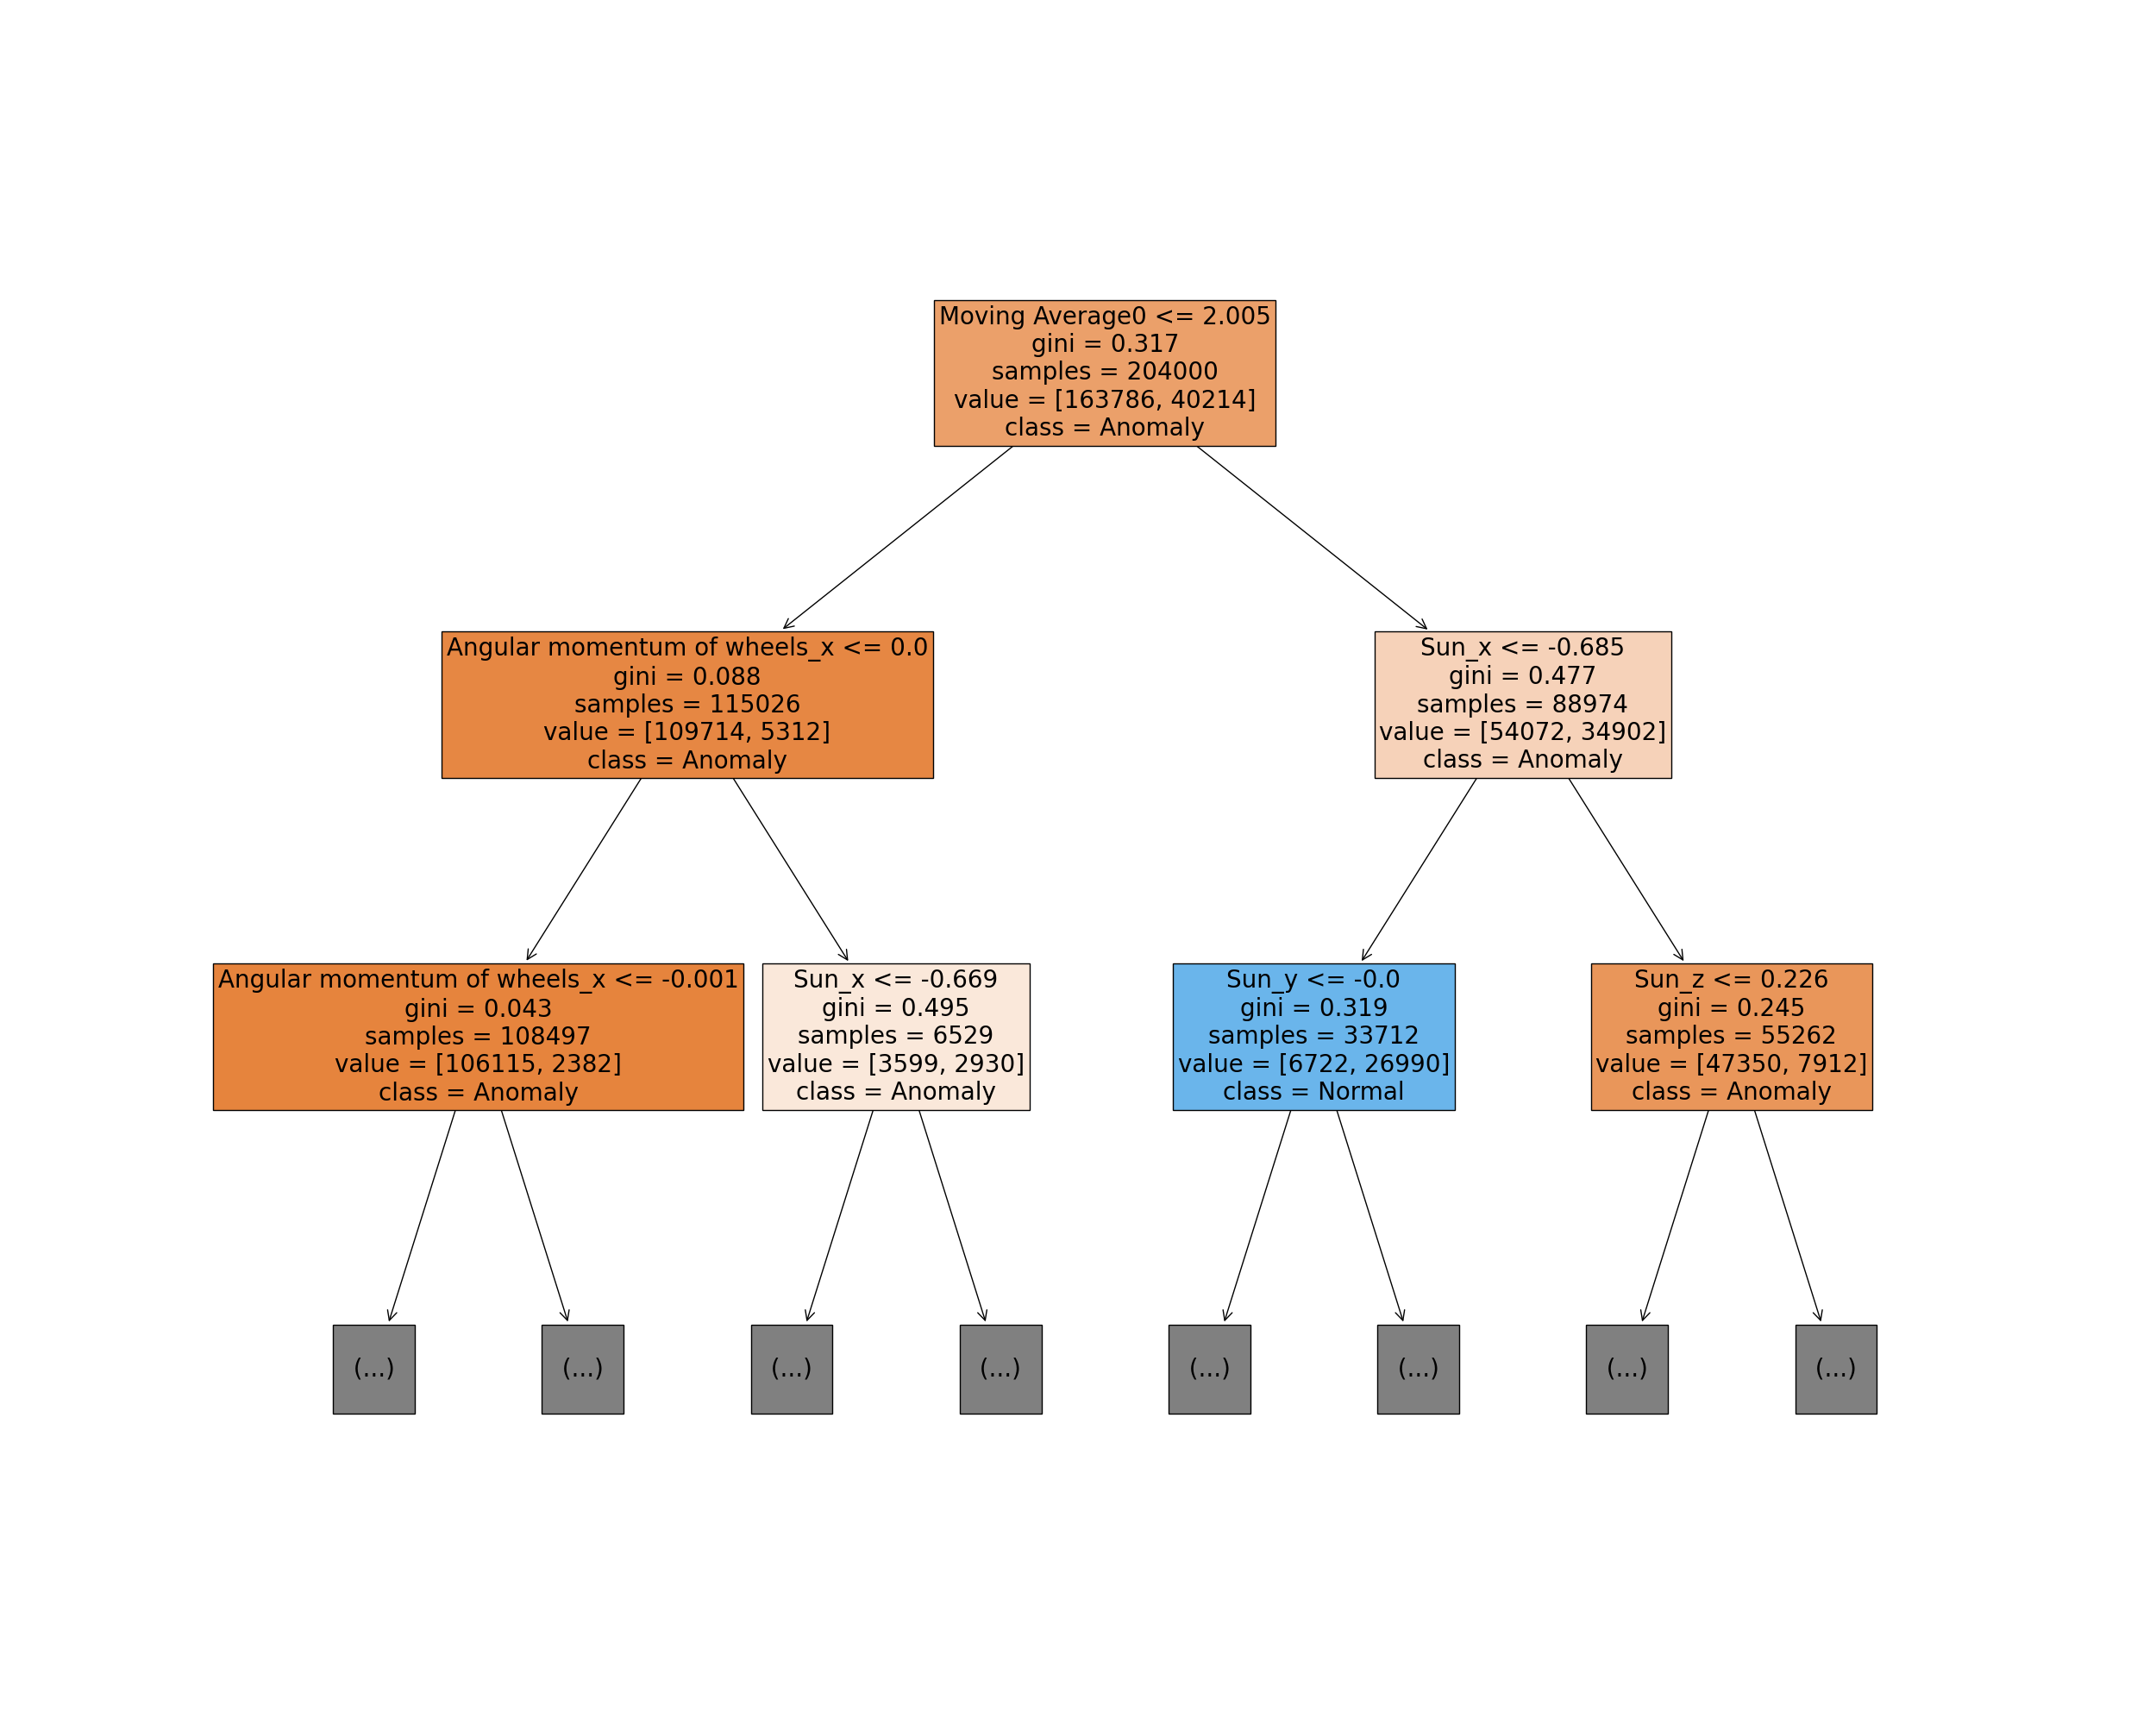
\includegraphics[trim = {4cm 8cm 4cm 8cm},clip, width = 15cm]{/home/ulrich/Documents/Masters thesis/Satellite/Hyperparameters/PhysicsEnabledDMDMethod/DecisionTreeBinaryClass.png}
	\caption{Decision Tree}
	\label{fig:DecisionTree}
\end{figure*}

It is evident in Figure~\ref{fig:DecisionTree} that the largest splits at the beginning of the tree is the moving average from the feature extraction as well as the sun sensor and angular momentum of the reaction wheels' measurements. This makes logical sense, since the moving average provides the system with an extracted feature that correlates the change in measurements. The sun reflection can also be detected on the sun sensor measurements and changes in the angular momentum of the wheels indicate that there could be large changes in the sun vector during the sun following period.

Random Forests, a method of using the prediction average of randomly sampled decision trees, is also tested and the results thereof shown in section~\ref{section:Results}.


\subsection{Recovery}
Three different methods of recovery are compared. These methods are all focused on ensuring that the sun reflection does not change the reliability and stability of the EKF.

The ignore method uses the detected sensor that has failed and ignores the sensor measurement from the EKF measurement update. This method is based on the assumption that the EKF estimation is correct up until the moment where the sensor failure is detected. This however will highly depend on the accuracy of the anomaly detection method. Since a detection method with low accuracy will create instability of the EKF, since many anomalous measurements will be included in the measurement update of the EKF.

%The replacement methodology changes $v_{meas,k}$ to $v_{est,k}$ at the timestep when the failure is detected. This method depends on the stability and accuracy of the EKF when the failure is detected and highly depends on the accuracy of the detection method. Although this seems to bypass the entire purpose of a measurement update, and might change the EKF's dependency to be more on the sensor than the model, even though the sensor measurement might not be accurate. The EKF will remain stable due to the other measurements being accurate and will save computation time. The EKF will not require any reset and the same number of measurements updates will still occur during a sensor's anomalous behaviour.

The backtrack method uses a buffer of $v_{meas,k}$, $v_{model,k}$ and $\hat{x}_k^+$ and other parameters that are used to update the EKF. If a sensor failure is detected, the sensor is excluded from the EKF and the EKF is updated with the sensor data in the buffer excluding the sensor that has failed. The EKF is therefore \emph{reset} and updated from timestep $t_{k-N}$ to $t_k$, where $N$ is the size of the number of timesteps in the buffer. $N$ however must be optimized based on the computational time used to reset the EKF, but still ensure convergence of the EKF. If the sensor that was detected to have anomalous behaviour changes back to normal again, the EKF will be reset once again and the sensor will only be included in the measurement update of $t_k$ since it was anomalous for timesteps before $t_k$.

A backtrack method can be combined with the ignore method. Where the backtrack method is implemented only after a specified number of sun reflections are predicted.

Another method implemented and tested always uses the two sensors measurements that has the smallest mean squared error between the estimated SBC vector and the actual measured SBC vector. There are setbacks to this method. Firstly, it requires the modelling of the ORC vector and requires the position of the satellite in orbit. Secondly, this method will not work with small drifts in a sensor measurement, since the estimator will latch unto the drift in the sensor. The method will only detect sudden changes in the sensor, but will isolated the sudden change even if it remains stable after the sudden change. This method is will only compared to the other methods as part of the analysis, since it the method is inherently different.

\section{Testing Setup}
To ensure repeatability of the tests conducted in this article, the sgp4 simulation environment is used for the position in orbit of the satellite. The disturbance torques modelled in this simulation is the aerodynamic disturbances, static and dynamic wheel disturbances, gravity gradient disturbances, and gyroscopic disturbances. The testing for the FDIR methods is done by implementing a reflection model on a cubesat from the moment of launching the satellite. Therefore the recovery methods are also implemented from the beginning of the satellite orbit. The mission of the ADCS of this specific satellite is to be nadir pointing during eclipse and sun following otherwise.

\subsection{Control}
Quaternion-feedback control with momentum dumping only during eclipse is implemented. The attitude command vector during nadir-pointing in the SBC frame is $\mathbf{u}_c = [0, 0, 1]$, since the SBC frame $z$ coordinate should line up with the ORC frame. During the sun following phase, the attitude command according to \textcite{chen2000ground} can be calculated as 

\begin{equation}
\mathbf{u}_c = \frac{\mathbf{u}_{sp}^{SBC} \times \mathbf{s}_o}{\norm{\mathbf{u}_{sp}^{SBC} \times \mathbf{s}_o}}
\end{equation}

where $\mathbf{s}_o$ is the measured unit sun vector in ORC, and the main solar panel's position is denoted as a unit vector, $\mathbf{u}_{sp}^{SBC}$. The angle between $\mathbf{u}_{sp}^{SBC}$ and $\mathbf{s}_o$, $\delta$, can be calculated with the vector dot-product. The command quaternion $\mathbf{q}_c$ can then be calculated

\begin{equation}
\mathbf{q}_c = \begin{bmatrix}
	\mathbf{u}_c sin(\frac{\delta}{2}) \\
	cos(\frac{\delta}{2})
\end{bmatrix}
\end{equation}
This can then be used as the reference for the control. The reference $\boldsymbol{\omega}_b^I$ is always $[0, 0, 0]$.

\subsection{Dimensions of Satellite}
The dimensions of the satellite are shown in Table~\ref{Table:Dimensions}. The dimensions are shown to ensure the repeatability of the results in this article. The dimensions of the sun sensor are from the Sputnix cubesat sun sensor model.

\begin{table}[!htb]
	\caption{\label{Table:Dimensions}Dimensions of Cubesat}
	\begin{tabular}{|c|c|c|c|}
		\hline
		\textbf{Dimensions} & \textbf{Satellite (m)} & \textbf{Solar Panels (m)} & \textbf{Sun Sensor (m)} \\ \hline
		\textbf{x}          & $0.3$                    & $0.3$                       & $0.028$                   \\ \hline
		\textbf{y}          & $0.3$                    & $0.3$                       & $0.023$                   \\ \hline
		\textbf{z}          & $0.4$                    & $0.002$                     & N/A                     \\ \hline
	\end{tabular}
\end{table}

% https://sputnix.ru/en/equipment/cubesat-devices/sun-sensor-flight-proof-1
% https://www.cubesatshop.com/product/nss-cubesat-sun-sensor/

\subsection{Orbit Parameters}
The orbit parameters will not significantly effect the results, however, for repeatability the general parameters for the orbit is given in Table~\ref{Table:OrbitParameters}. 
	
\begin{table}[!htb]
	\caption{\label{Table:OrbitParameters}Parameters for Cubesat Orbit}
	\begin{tabular}{|c|c|}
		\hline
		\textbf{Revolutions per day}          & $15.2355$                    \\ \hline
		\textbf{Inclination}          & $97.4^o$                    \\ \hline
		\textbf{Right ascension of the ascending node} & $275^o$ \\ \hline
	\end{tabular}
\end{table}

\subsection{Sensors}
The measurement update of the Kalman filter will firstly be with a magnetometer, nadir sensor and lastly the sun sensor. This is due to the noise models of the sensors, as all the sensor noise models are based on zero-mean Guassian random noise and the magnetometer has the largest standard deviation and the sun sensor has the smallest standard deviation. There are two sun sensors, a coarse and fine sun sensor and both of them can experience sun reflection. The field of view \emph{FOV} of the sun sensors and the nadir sensor are both $180^o$. There is however only a single nadir sensor used in the simulation.

\section{Results}
\label{section:Results}
Three scenarios are implemented, a satellite that never experiences reflection, a satellite that experiences reflection without any recovery method and a satellite with a recovery method. The subsets of detecting the fault and recovering from the fault will be isolated and discussed separately. Therefore the results for recovery based on perfect detection can be shown to provide the theoretical possibilities of the recovery method. Please note that the scale of the y-axis for each plot is not the same due to the large differences between the maximum y-values for each scenario.

The pointing metric is the difference between the command or reference attitude and the actual attitude in degrees. The estimation metric is the difference between the actual attitude and the estimated attitude in degrees.

\subsection{Perfect Designed Satellite Without Reflection}
This test is implemented for the current design with the assumption that the sun sensor will never experience sun reflection. This also indicates the best scenario for the ADCS and requires a well designed satellite. The results for the first 5 orbits are shown to provide a desired result for the recovery methods as shown in Figure~\ref{fig:Pointing Accuracy None} and Figure~\ref{fig:Estimation Accuracy None}. 
\begin{figure}[!htb]
	\begin{center}
		\import{Figures/TexFigures/Predictor-None/Isolator-None/Recovery-None/EARTH_SUN-ORC-General CubeSat Model/None/}{Pointing Metric.pgf}
	\end{center}
	\caption[Pointing Metric for Satellite Without Reflection]{Pointing Metric for Satellite Without Reflection.}
	\label{fig:Pointing Accuracy None}
\end{figure}

\begin{figure}[!htb]
	\begin{center}
	\import{Figures/TexFigures/Predictor-None/Isolator-None/Recovery-None/EARTH_SUN-ORC-General CubeSat Model/None/}{Estimation Metric.pgf}
	\end{center}
	\caption[Estimation Metric for Satellite Without Reflection]{Estimation Metric for Satellite Without Reflection.}
	\label{fig:Estimation Accuracy None}
\end{figure}

From Figure~\ref{fig:Pointing Accuracy None} it evidently shows the transition of the reference vector between the eclipse and sunlit phases. This is the reason for the spikes in the point metric at the beginning of each period. From Figure~\ref{fig:Estimation Accuracy None} it is also evident that the estimation is more accurate during the sunlit phase, which correlates with the fact that the sun sensor has a smaller noise.

\subsection{Satellite With Reflection}
If no recovery strategy is implemented for the reflection anomaly, the EKF is very unstable and the estimation is very inaccurate. As a bare minimum the proposed methods should be have a lower pointing and estimation metric than the results shown in Figure~\ref{fig:Pointing Accuracy Reflection} and Figure~\ref{fig:Estimation Accuracy Reflection}. It is clear that the ADCS is unstable and the average estimation metric of a satellite without reflection is compared to the various recovery methods in Figure~\ref{fig:Estimation Metric Summary}.

\begin{figure}[!htb]
	\begin{center}
	\import{Figures/TexFigures/Predictor-None/Isolator-None/Recovery-None/EARTH_SUN-ORC-General CubeSat Model/Reflection/}{Pointing Metric.pgf}
	\end{center}
	\caption[Pointing Metric for Satellite with Reflection and without FDIR]{Pointing Metric for Satellite with Reflection and without FDIR.}
	\label{fig:Pointing Accuracy Reflection}
\end{figure}

\begin{figure}[!htb]
	\begin{center}
	\import{Figures/TexFigures/Predictor-None/Isolator-None/Recovery-None/EARTH_SUN-ORC-General CubeSat Model/Reflection/}{Estimation Metric.pgf}
	\end{center}
	\caption[Estimation Metric for Satellite with Reflection and without FDIR]{Estimation Metric for Satellite with Reflection and without FDIR.}
	\label{fig:Estimation Accuracy Reflection}
\end{figure}

\subsection{Perfect Detection}
This section indicates the results for each recovery method, with the assumption that the detection method is perfect. This means that the detection methodology will produce an accuracy of $100\%$. This is used to determine which method is most suitable for recovery from sensor anomalies since it provides the theoretical best scenario for each method. The mean estimation for each orbit is shown in Figure~\ref{fig:Estimation Metric Summary} and it is evident that the EKF-ignore method is the method that reduces the estimation error the most during a period of $30$ orbits. 

\begin{figure}[!htb]
	\begin{center}
		\import{Figures/TexFigures/Summary/PERFECT/}{Estimation Metric.pgf}
	\end{center}
	\caption[Estimation Metric for Perfect Detection]{Estimation Metric for Perfect Detection.}
	\label{fig:Estimation Metric Summary}
\end{figure}

Due to the significant difference in performance between the EKF-ignore and the other recover methods, only the EKF-ignore method will be further investigated with other detection strategies.

\subsection{Satellite With Recovery Ignore}
To show the promising results of the recovery ignore for perfect detection Figure~\ref{fig:Estimation Accuracy EKF-ignore} shows the estimation metric during the first 5 orbits. Our goal is to introduce detection strategies that produce similar results.

\begin{figure}[!htb]
	\begin{center}
		\import{Figures/TexFigures/Predictor-PERFECT/Isolator-OnlySun/Recovery-EKF-ignore/EARTH_SUN-ORC-General CubeSat Model/Reflection/}{Estimation Metric.pgf}
	\end{center}
	\caption[Estimation Metric for Satellite with Recovery Ignore]{Estimation Metric for Satellite with Recovery Ignore.}
	\label{fig:Estimation Accuracy EKF-ignore}
\end{figure}


\begin{figure}[!htb]
	\begin{center}
		\import{Figures/TexFigures/Summary/EKF-ignore/}{Estimation MetricRandomForestDifferentDepths.pgf}
	\end{center}
	\caption[Estimation Metric for Different Depths of RandomForests]{Estimation Metric for Different Depths of RandomForests.}
	\label{fig:Estimation Accuracy EKF-ignore RandomForest depth}
\end{figure}

\begin{figure}[!htb]
	\begin{center}
		\import{Figures/TexFigures/Summary/EKF-ignore/}{Estimation MetricDecisionTreesDifferentDepths.pgf}
	\end{center}
	\caption[Estimation Metric for Different Depths of RandomForests]{Estimation Metric for Different Depths of RandomForests.}
	\label{fig:Estimation Accuracy EKF-ignore Decision Tree depth}
\end{figure}

To compare the results between the detection methods the mean estimation metric for 30 orbits are shown in Figure~\ref{fig:Estimation Accuracy EKF-ignore summary}. It is clear that both the Decision Tree and the Random Forest method as detection methods for the EKF-ignore produce better results than a satellite without any FDIR as shown in Figure~\ref{fig:Estimation Metric Summary}. 

\begin{figure}[!htb]
	\begin{center}
		\import{Figures/TexFigures/Summary/EKF-ignore/}{Estimation Metric.pgf}
	\end{center}
	\caption[Estimation Metric for Satellite with Recovery Ignore and Various detection Methods]{Estimation Metric for Satellite with Recovery Ignore and Various Detection Methods.}
	\label{fig:Estimation Accuracy EKF-ignore summary}
\end{figure}

However from Figure~\ref{fig:Estimation Accuracy EKF-ignore summary} it is clear that our estimation is not as we desired. The confusion matrix for both Random Forest and Decision Trees from Table~\ref{Table: Prediction Accuracy-DMDRandomForestOnlySunEKF-ignoreReflection-Reflection} and Table~\ref{Table: Prediction Accuracy-DMDDecisionTreesOnlySunEKF-ignoreReflection-Reflection} respectively indicates that the methods are able to predict the failures and no failures with more or less the same percentage false positives and negatives. The Random Forest has false positives of $15\%$ compared to the false negatives of $10\%$, while Decision Trees have a false positive percentage of $16.1\%$ and a false negative percentage of $18.7\%$. However both these methods has more or less the same estimation error during the 30 orbits.

\import{Tables/Prediction Accuracy/}{Prediction Accuracy-DMDRandomForestOnlySunEKF-ignoreReflection-Reflection.tex}

\import{Tables/Prediction Accuracy/}{Prediction Accuracy-DMDDecisionTreesOnlySunEKF-ignoreReflection-Reflection.tex}

Due to the results from the confusion matrices, we want to do an analysis of what is required for a suitable detection strategy. In Figure~\ref{fig:Prediction Accuracy EKF-ignore summary} we can see what the percentage values are to produce an estimation error as shown in Figure~\ref{fig:Estimation Accuracy EKF-ignore summary}. To do a comparison we used a uniform random generator to produce accuracies of fixed percentages as shown in the legend of Figure~\ref{fig:Estimation Accuracy EKF-ignore Comparison}. This figure clearly indicates that any percentage accuracy less than $99.0\%$ produces an average estimation error of more than $20^o$. 

\begin{figure}[!htb]
	\begin{center}
		\import{Figures/TexFigures/Summary/EKF-ignore/}{Prediction Accuracy.pgf}
	\end{center}
	\caption[Prediction Accuracy of Various Methods]{Prediction Accuracy of Various Methods.}
	\label{fig:Prediction Accuracy EKF-ignore summary}
\end{figure}


\begin{figure}[!htb]
	\begin{center}
		\import{Figures/TexFigures/Summary/EKF-ignore/}{Estimation MetricPerfectNoFailurePrediction.pgf}
	\end{center}
	\caption[Estimation Metric of Fixed Percentage Accuracies During Failures and Perfect Prediction During No Failures]{Estimation Metric of Fixed Percentage Accuracies During Failures and Perfect Prediction During No Failures.}
	\label{fig:Estimation Accuracy EKF-ignore Comparison PerfectNoFailure}
\end{figure}

\begin{figure}[!htb]
	\begin{center}
		\import{Figures/TexFigures/Summary/EKF-ignore/}{Estimation MetricComparison-Standard.pgf}
	\end{center}
	\caption[Estimation Metric of Fixed Percentage Accuracy]{Estimation Metric of Fixed Percentage Accuracy.}
	\label{fig:Estimation Accuracy EKF-ignore Comparison}
\end{figure}

\begin{figure}[!htb]
	\begin{center}
		\import{Figures/TexFigures/Summary/EKF-ignore/}{Estimation MetricEKF-top2PerfectNoFailurePrediction.pgf}
	\end{center}
	\caption[Estimation Metric of Fixed Percentage Accuracies During Failures and Perfect Prediction During No Failures with Recovery Buffer]{Estimation Metric of Fixed Percentage Accuracies During Failures and Perfect Prediction During No Failures with Recovery Buffer.}
	\label{fig:Estimation Accuracy EKF-ignore PerfectNoFailure with Recovery Buffer}
\end{figure}

\begin{figure}[!htb]
	\begin{center}
		\import{Figures/TexFigures/Summary/EKF-ignore/}{Estimation MetricEKF-top2.pgf}
	\end{center}
	\caption[Estimation Metric of Fixed Percentage Accuracy with Recovery Buffer]{Estimation Metric of Fixed Percentage Accuracy with Recovery Buffer.}
	\label{fig:Estimation Accuracy EKF-ignore with Recovery Buffer}
\end{figure}

\begin{figure}[!htb]
	\begin{center}
		\import{Figures/TexFigures/Predictor-90.0/Isolator-OnlySun/Recovery-EKF-ignore/EARTH_SUN-ORC-General CubeSat Model/Reflection/}{Estimation Metric.pgf}
	\end{center}
	\caption[Estimation Metric of $90.0\%$ Accuracy]{Estimation Metric of Fixed Percentage Accuracy.}
	\label{fig:Estimation Accuracy EKF-ignore 90}
\end{figure}

\begin{figure}[!htb]
	\begin{center}
		\import{Figures/TexFigures/Predictor-90.0/Isolator-OnlySun/Recovery-EKF-ignore/EARTH_SUN-ORC-General CubeSat Model/ReflectionPerfectNoFailurePrediction/}{Estimation Metric.pgf}
	\end{center}
	\caption[Estimation Metric of $90.0\%$ Accuracy]{Estimation Metric of Fixed Percentage Accuracy.}
	\label{fig:Estimation Accuracy EKF-ignore 90 perfectnofailureprediction}
\end{figure}

\begin{figure}[!htb]
	\begin{center}
		\import{Figures/TexFigures/Predictor-90.0/Isolator-OnlySun/Recovery-EKF-ignore/EARTH_SUN-ORC-General CubeSat Model/ReflectionEKF-top2/}{Estimation Metric.pgf}
	\end{center}
	\caption[Estimation Metric of $90.0\%$ Accuracy with Recovery Buffer]{Estimation Metric of Fixed Percentage Accuracy with Recovery Buffer.}
	\label{fig:Estimation Accuracy EKF-ignore 90 with Recovery Buffer}
\end{figure}

\begin{figure}[!htb]
	\begin{center}
		\import{Figures/TexFigures/Predictor-90.0/Isolator-OnlySun/Recovery-EKF-ignore/EARTH_SUN-ORC-General CubeSat Model/ReflectionEKF-top2/PerfectNoFailurePrediction/}{Estimation Metric.pgf}
	\end{center}
	\caption[Estimation Metric of $90.0\%$ Accuracy]{Estimation Metric of Fixed Percentage Accuracy.}
	\label{fig:Estimation Accuracy EKF-ignore 90 perfectnofailureprediction with Recovery Buffer}
\end{figure}


\subsection{First Order Filter}
The $99.0\%$ prediction accuracy is a tall order for any prediction method. Therefore we test a method that only uses the two sensors who's measurement is the closest to the estimated vectors from the EKF and the modelled ORC vectors. This method will be name EKF-top2 for ease of reference. From this we are able to produce a results similar to a $99.0\%$ accuracy with the EKF-ignore method.

\begin{figure}[!htb]
	\begin{center}
		\import{Figures/TexFigures/Summary/EKF-top2/}{Estimation Metric.pgf}
	\end{center}
	\caption[Estimation Metric for Satellite with Recovery Ignore and Various detection Methods]{Estimation Metric for Satellite with Recovery Ignore and Various Detection Methods.}
	\label{fig:Estimation Accuracy EKF-top2 summary}
\end{figure}

\begin{figure}[!htb]
	\begin{center}
		\import{Figures/TexFigures/Summary/RandomForest100/}{Estimation Metric.pgf}
	\end{center}
	\caption[Estimation Metric of RandomForest with Recovery Buffer]{Estimation Metric of RandomForest with Recovery Buffer.}
	\label{fig:Summary Estimation Accuracy EKF-ignore RandomForest with Recovery Buffer}
\end{figure}

\begin{figure}[!htb]
	\begin{center}
		\import{Figures/TexFigures/Predictor-RandomForest100/Isolator-OnlySun/Recovery-EKF-ignore/EARTH_SUN-ORC-General CubeSat Model/ReflectionEKF-top2/}{Estimation Metric.pgf}
	\end{center}
	\caption[Estimation Metric of RandomForest with Recovery Buffer]{Estimation Metric of RandomForest with Recovery Buffer.}
	\label{fig:Estimation Accuracy EKF-ignore RandomForest with Recovery Buffer}
\end{figure}

\begin{figure}[!htb]
	\begin{center}
		\import{Figures/TexFigures/Predictor-RandomForest100/Isolator-OnlySun/Recovery-EKF-ignore/EARTH_SUN-ORC-General CubeSat Model/Reflection/}{Estimation Metric.pgf}
	\end{center}
	\caption[Estimation Metric of $90.0\%$ Accuracy with Recovery Buffer]{Estimation Metric of Fixed Percentage Accuracy with Recovery Buffer.}
	\label{fig:Estimation Accuracy EKF-ignore RandomForest withoutt Buffer}
\end{figure}

\begin{figure}[!htb]
	\begin{center}
		\import{Figures/TexFigures/Predictor-RandomForest100/Isolator-OnlySun/Recovery-EKF-ignore/EARTH_SUN-ORC-General CubeSat Model/ReflectionEKF-top2/PerfectNoFailurePrediction/}{Estimation Metric.pgf}
	\end{center}
	\caption[Estimation Metric of $90.0\%$ Accuracy with Recovery Buffer and Prefect No Failure Prediction]{Estimation Metric of Fixed Percentage Accuracy with Recovery Buffer and Prefect No Failure Prediction.}
	\label{fig:Estimation Accuracy EKF-ignore 90 with Recovery Buffer and prefectNoFailurePrediction}
\end{figure}

Even though the EKF-top2 method performs as well as a $99.0\%$ accuracy, it will decrease the performance of a system where no sun reflection ever occurs. Due to it not utilizing all three of the sensors during the measurement update. Therefore, further analysis must be done on combining the EKF-top2 method with the EKF-ignore method and only utilizing the EKF-top2 method when there is significant uncertainty. 

An idea for further analysis is to use a threshold for the percentage uncertainty of the prediction and when the uncertainty is within a given range then the EKF-top2 method will be implemented. Another possible derivation of the current detection methods is to use the state covariance values from the EKF and then backtracking the measurement updates. This prediction will be more accurate due to the sudden change in the state covariance matrix due to the anomalous sensor.

\section{CONCLUSIONS}
Before written the conclusion do a further analysis of the ideas in the previous paragraph.

\addtolength{\textheight}{-12cm}   % This command serves to balance the column lengths
                                  % on the last page of the document manually. It shortens
                                  % the textheight of the last page by a suitable amount.
                                  % This command does not take effect until the next page
                                  % so it should come on the page before the last. Make
                                  % sure that you do not shorten the textheight too much.

%%%%%%%%%%%%%%%%%%%%%%%%%%%%%%%%%%%%%%%%%%%%%%%%%%%%%%%%%%%%%%%%%%%%%%%%%%%%%%%%



%%%%%%%%%%%%%%%%%%%%%%%%%%%%%%%%%%%%%%%%%%%%%%%%%%%%%%%%%%%%%%%%%%%%%%%%%%%%%%%%

% \begin{thebibliography}{99}

% \bibitem{c1} G. O. Young, ÒSynthetic structure of industrial plastics (Book style with paper title and editor),Ó 	in Plastics, 2nd ed. vol. 3, J. Peters, Ed.  New York:  % McGraw-Hill, 1964, pp. 15Ð64.
% \bibitem{c2} W.-K. Chen, Linear Networks and Systems (Book style).	Belmont, CA: Wadsworth, 1993, pp. 123Ð135.

\printbibliography[heading=bibintoc]




% \end{thebibliography}



\end{document}
